\chapter{Rotation of the Hand UI Model}

\label{Chapter4_rotation} 

\begin{comment}
-------------------------------------------------
%								Chapter layout
4. Rotation of Hand UI Model
	a. Description of Problem
	a. JavaFx Coordinate System vs Leap Motion Coordinate System
	b. Ineffective Leap Motion Data
		i. Pitch Roll Yaw
		ii. Negative Zeros
	c. Simplified Hand Model
	d. Composite Linear Transformations
	e. Rotational Matrix
-------------------------------------------------
\end{comment}
In this chapter the rotation of the Hand UI model will be discussed. 

%------------------------------------------------
%	SECTION 1 Description of Problem
%------------------------------------------------
\section{Description of Problem}
The UI model of the hand is built from the Leap Motion sensor data as discussed in the chapter. This data represents the hand as it is displayed in reality above the Leap Motion controller device. Originally the representation of the hand was built from this hand without any further modifications. However, to demonstrate why this is sometimes not the ideal situation, see Figure \ref{fig:handFlat}. It shows the hand as it is displayed in reality; it is in parallel plane above the device. 
\begin{figure}[H]
\centering
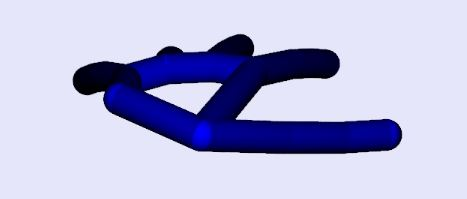
\includegraphics[scale=0.45]{Figures/4_handFlat.JPG}
\caption[Hand in Flat Orientation]{This shows the user's hand in a flat orientation; as determined by the Leap Motion sensor.}
\label{fig:handFlat}
\end{figure}
It should noted how difficult it is to see the fingers and thumb. They are only barely visible. Therefore the user would be forced to force his or her hand into a vertical postion by straining their wrist just so they can see the gesture they are performing on the screen. Figures \ref{fig:handYaw} and \ref{fig:handRoll} show other orientation the hand can take; these figures show the hand after a yaw rotation and after a roll rotation respectively. Again, note the slight difficulty in figuring out the thumb and fingers positions and orientations when the hand is rolled around the z-axis. The hand that is shown in the yaw rotation in Figure \ref{fig:handYaw} is able to seen a little clearly because the wrist was strained upwards. 
\begin{figure}[H]
    \centering
    \begin{minipage}{0.5\textwidth}
        \centering
        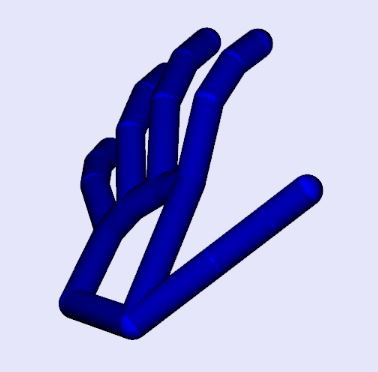
\includegraphics[scale=.55]{Figures/4_handYaw.JPG} 
        \caption[Hand with Yaw Rotation]{The user's hand after the certain yaw rotation around the y-axis.}
		\label{fig:handYaw}
    \end{minipage}\hfill
    \begin{minipage}{0.5\textwidth}
        \centering
        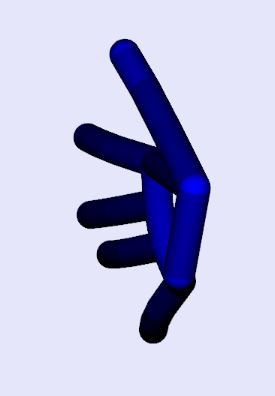
\includegraphics[scale=.55]{Figures/4_handRoll.JPG}
        \caption[Hand with Roll Rotation]{The user's hand after the certain roll rotation around the z-axis.}
        \label{fig:handRoll}
    \end{minipage}
\end{figure}
Finally all of these different orientation can of course overlap with each other to create a complex orientation of the hand as shown in Figure \ref{fig:weirdHandShake}, which shows the user's left hand in a weird handshake sort of position while being rotated to the right and tilted upwards.
\begin{figure}[H]
\centering
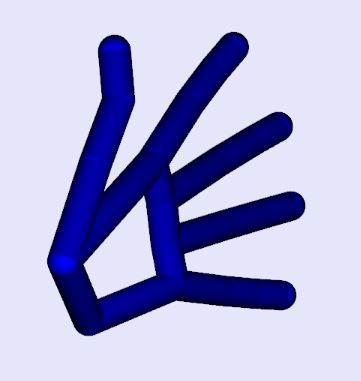
\includegraphics[scale=0.45]{Figures/4_handWeirdHandshake.JPG}
\caption[Hand in Weird Handshake Position]{This shows the user's hand in a flat orientation; as determined by the Leap Motion sensor.}
\label{fig:weirdHandShake}
\end{figure}
This chapter will explain how these different possible orientations the user's hand might be in while they are performing gestures shown on the screen are accounted for and "undone". Doing this results in the user's hand to be displayed in a set vertical orientation on the screen despite the different ways the user may have oriented their hand above the device in reality. The final resulting hand for all of the figures seen previously  will be as is shown in Figure \ref{fig:handFinalResult} after the composite rotation have transformed it to a vertical position. 
\begin{figure}[H]
\centering
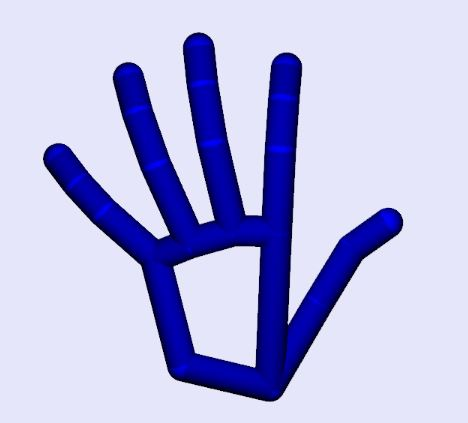
\includegraphics[scale=0.45]{Figures/4_handFinalFix.JPG}
\caption[Hand Fixed to Vertical Orientation]{This shows what the user's hand will look like after all of the possible rotational transforms have been undone and the hand has been fixed to a vertical orientation.}
\label{fig:weirdHandShake}
\end{figure}
This feature of the application makes it easier for the user to see what his or her hand is doing without requiring them to always contain their hand in a specific orientation. The goal of this application is to measure the accuracy with which a user is able to complete certain gestures, not the orientation of their hand. In fact, the algorithms that are used to grade the correctness of the user's attempted gesture do not take the user's hand orientation into account. They focus on the fingers bones and their relative orientations to each other. At the beginning of this project, one of the ideas discussed was to build some sort of rig which would be used to place the user's hand in a set orientation. However because of what will be explained in this chapter such a rig is no longer necessary.



%------------------------------------------------
%	SECTION 1 JavaFx CS vs Leap Motion CS
%------------------------------------------------
\section{JavaFx Coordinate System vs Leap Motion Coordinate System}
The Leap Motion controller has a different coordinate system from JavaFX. This distinction is very important to get out of the way as the rest of the chapter will rely on such an understanding. The coordinate system for the Leap Motion device is shown in Figure \ref{fig:leapcs}. Note the placement of the green LED light in the Leap Motion device as shows the orientation of the otherwise symetrical picture.
\begin{figure}[H]
\centering
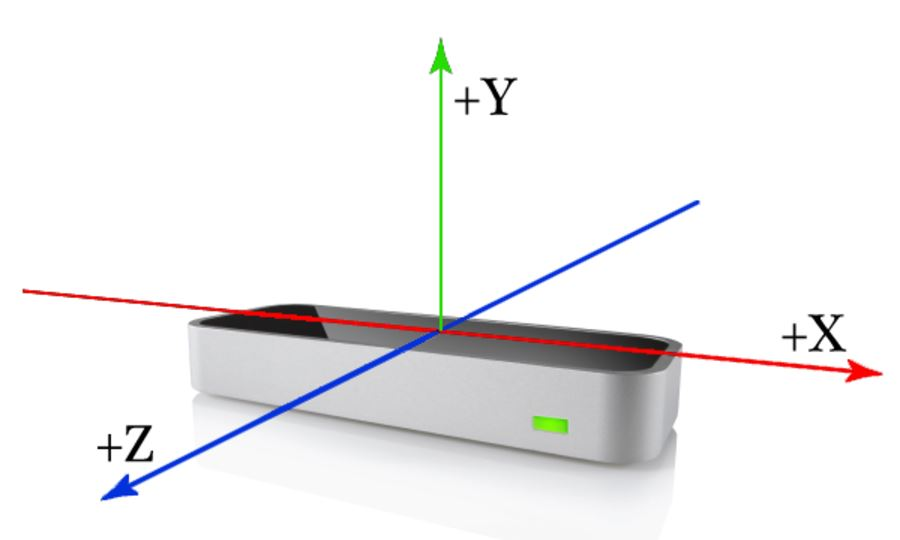
\includegraphics[scale=0.35]{Figures/4_leapCS.JPG}
\caption[Leap Motion Coordinate System]{The coordinate system that is used by the Leap Motion sensor. Data collected will based upon these axes.}
\label{fig:leapcs}
\end{figure}

This coordinate system is referred to as a right-handed coordinate system because of the easy way in which it can be represented by the first three fingers of the right hand as shown in Figure \ref{fig:lhcsRhcs}. 
\begin{figure}[H]
\centering
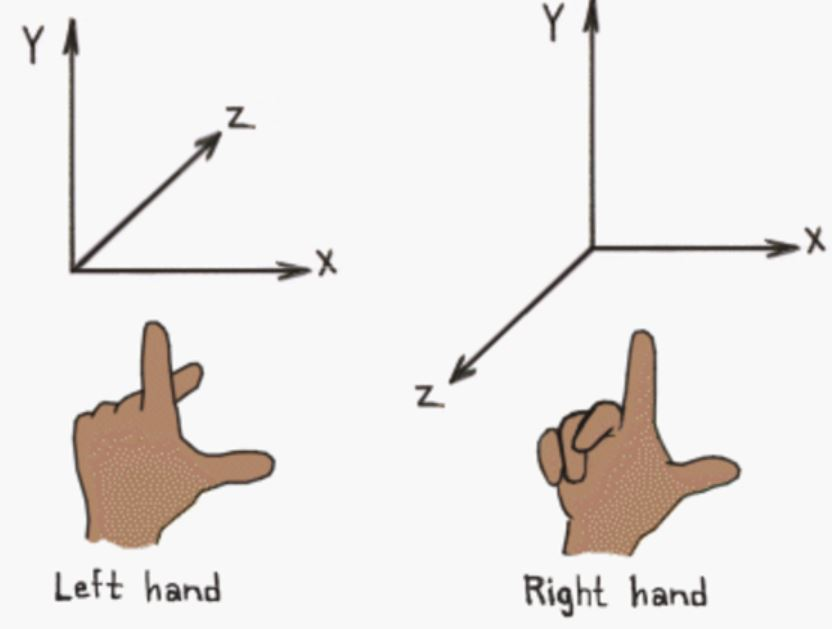
\includegraphics[scale=0.35]{Figures/4_lhrhCS.JPG}
\caption[Left vs Right Hand Coordinate System]{Left and right handed coordinate systems and how they can be shown via fingers.}
\label{fig:lhcsRhcs}
\end{figure}

In contrast, the traditional coordinate system which is used in computer science and which is what JavaFX also follows is shown in Figure \ref{fig:javafxcs}. The JavaFx coordinate system is not left handed or right handed as far as we can tell from the Figures shown. 
\begin{figure}[H]
\centering
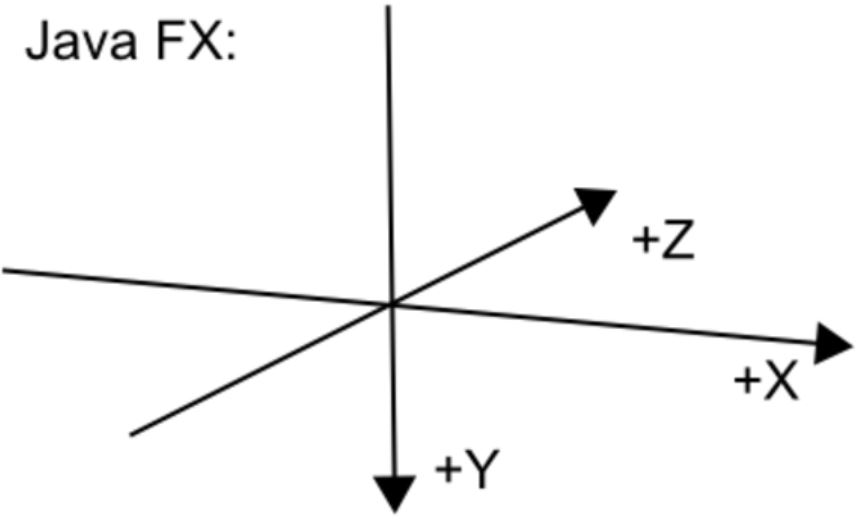
\includegraphics[scale=0.35]{Figures/4_javafxCS.JPG}
\caption[JavaFX Coordinate System]{The coordinate system used in JavaFX. Setting transforms on objects will be based on this coordinate system.}
\label{fig:javafxcs}
\end{figure}

Understanding these somewhat subtle difference and being able to switch from one context to the other was very important when considering the various rotational transforms that needed to be applied to the Hand UI model in order to straighten it to a vertical position. For example, one of the things that caused me some headaches sometimes when I was fixing and debugging my code was the fact that 3D rotations are measured in a very specific way. When it is said that some object is rotated around the y-axis by 90 degrees, this means that the if we imagine ourselves to be an observer standing on the y-axis and looking down the negative direction of this y-axis, then we would observe the object to rotate counter-clockwise about the y-axis. Therefore, it becomes very clear why it is significant to have clear understanding of the coordinate system that is being used for a particular section of code. Leap Motion data is returned with the default settings of the Leap Motion coordinate system. This data must be appropriately modified when the code using it is based upon the JavaFX coordinate system. Likewise composite rotations around certain axis might become jumbled up if one is not careful.  	


%------------------------------------------------
%	SECTION 2 Unexpected Leap Motion API Results 
%------------------------------------------------
\section{Unexpected Leap Motion API Results} 
In the course of working on this feature, which was explained in first section of this chapter, I realized that I was being returned results from the Leap Motion API that I was not expecting. I tested and debugged further into these issues until I realized some interesting things about the Leap Motion API which helped me to implement the vertical rotation of the user's hand successfully. In this section, I will go over some of the unexpected results that I obtained when I was learning more about the Leap Motion API's. I created a speciall Java class to help me in this endeaver which contains code samples with some simple yet illustrative scenarios which show how the Leap Motion API works. 






that some of the which I believed to be very simple scenarios  

- discuss the problem found in debug helper. 
- explain how you tried to do something very simple but the result surprised you. explain that here. 

- pyr are on vectors. explain via vectors. the problem below. 
- then explain the problem a little more in depth in terms of pry. and how they are not based on the wrist and palm. but rather on z-axis. 
- and how they are not returning good values. 

- can go a little bit into neg. zeros and how you solved this problem. 

- 
%----------------------------------- Pitch Roll Yaw
\subsection{Pitch Roll Yaw}


%----------------------------------- Negative Zeros
\subsection{Negative Zeros}




%------------------------------------------------
%	SECTION 3 Simplified Hand Model
%------------------------------------------------
\section{Simplified Hand Model}
	
	
%------------------------------------------------
%	SECTION 4 Composite Linear Transformations
%------------------------------------------------
\section{Composite Linear Transformations}




%------------------------------------------------
%	SECTION 5 Rotational Matrix
%------------------------------------------------
\section{Rotational Matrix}





